\documentclass[a4paper,12pt]{report}

\usepackage[utf8]{inputenc}
\usepackage[T1]{fontenc}
\usepackage{array}
\usepackage{amsmath}
\usepackage[english]{babel}
\usepackage{graphicx}
\usepackage[a4paper]{geometry}
\usepackage[colorlinks=true,urlcolor=blue,linkcolor=blue]{hyperref}
\usepackage{url}
\usepackage[nottoc,numbib]{tocbibind}
\usepackage{color}
\usepackage{epstopdf}
\usepackage{xcolor}
\usepackage[backend=biber,style=phys]{biblatex}
\usepackage{lipsum}
\usepackage[capbesideposition={right,center}]{floatrow}

\addbibresource{../Bibliography.bib}
\makeatletter
	\renewcommand{\thechapter}{\Roman{chapter}}
\makeatother

\newcolumntype{M}[1]{>{\centering\arraybackslash}m{#1}}

\floatsetup[table]{style=plaintop}

\begin{document}

\chapter{Growth of Cr-doped CdTe quantum dots\label{Growth}}

%	The growth took place at Tsukuba University, in the team of Pr. Shinji Kuroda. The samples were grown with Molecular Beam Epitaxy (MBE) and Atomic Layer Epitaxy (ALE, for the QD layer), via individual Cd, Te, Zn, Mg and Cr cells. MBE and ALE are two complementary techniques for the growth of semiconductor device.

	We studied to type of quantum dots: self assembled QDs, which have remaining strain on it, and strain free QDs. The strained dots are formed by the relaxation of a CdTe layer on ZnTe. Strain free dots are formed by thickness variation of a CdTe quantum well between CdMgTe barriers.
	
	\section{Generality on Molecular Beam Expitaxy}	
	
	The sample were grown using Molecular Beam Epitaxy (MBE). Cells of pure elements are heated to control their evaporation or until they reach sublimation. Those elements will formed the desired crystal on the substrate. They are kept in Knudsen cell, which consist of a crucibles of high-melting-point material with a low contaminating power (typically Pyrolytic Boron Nitride) wrapped in tungsten filament which will act as heater. Each are closed by a shutter controlled by a computer.
	
	Upon reaching the right temperature, said shutter is opened to let the element travel to the substrate. The the camber containing the substrate is kept in Ultra High Vacuum (about $10^{-8}$ Pa), in order to avoid contamination of the sample and get a mean free path of the gas long compared to distance to the sample. This process is illustrated on Fig.~\ref{MBEScheme}. Reaching the surface, the atoms diffuse before stopping, either having dissipated their kinetic through interaction with the surface, or (more commonly) being kept by island of previously deposited atoms. In the ideal case, the growth occur layer by layer, slowly (about 1 monolayer/s), giving a good control of the thickness of the grown material.
		
%	 This technique consist of heating cells containing the pure elements which will formed the semiconductor in order to sublimate or evaporate them, such as presented on Fig \ref{MBEScheme}. Once the element is at the right temperature, the cell is opened and the gas can travel in the chamber with a ballistic trajectory. The mean free path of this gas is long compared to the size of the cells and the chamber, allowing the atoms to condensate on the substrate without interacting before. Once reaching the surface, the atoms diffuse on it before stopping, either having dissipated their kinetic through interaction with the surface, or (more commonly) being kept by island of previously deposited atoms. In the ideal case, the growth occur layer by layer, slowly (about 1 monolayer/s), giving a good control of the thickness of the grown material.	

	\begin{figure}[h!]
	\begin{center}
		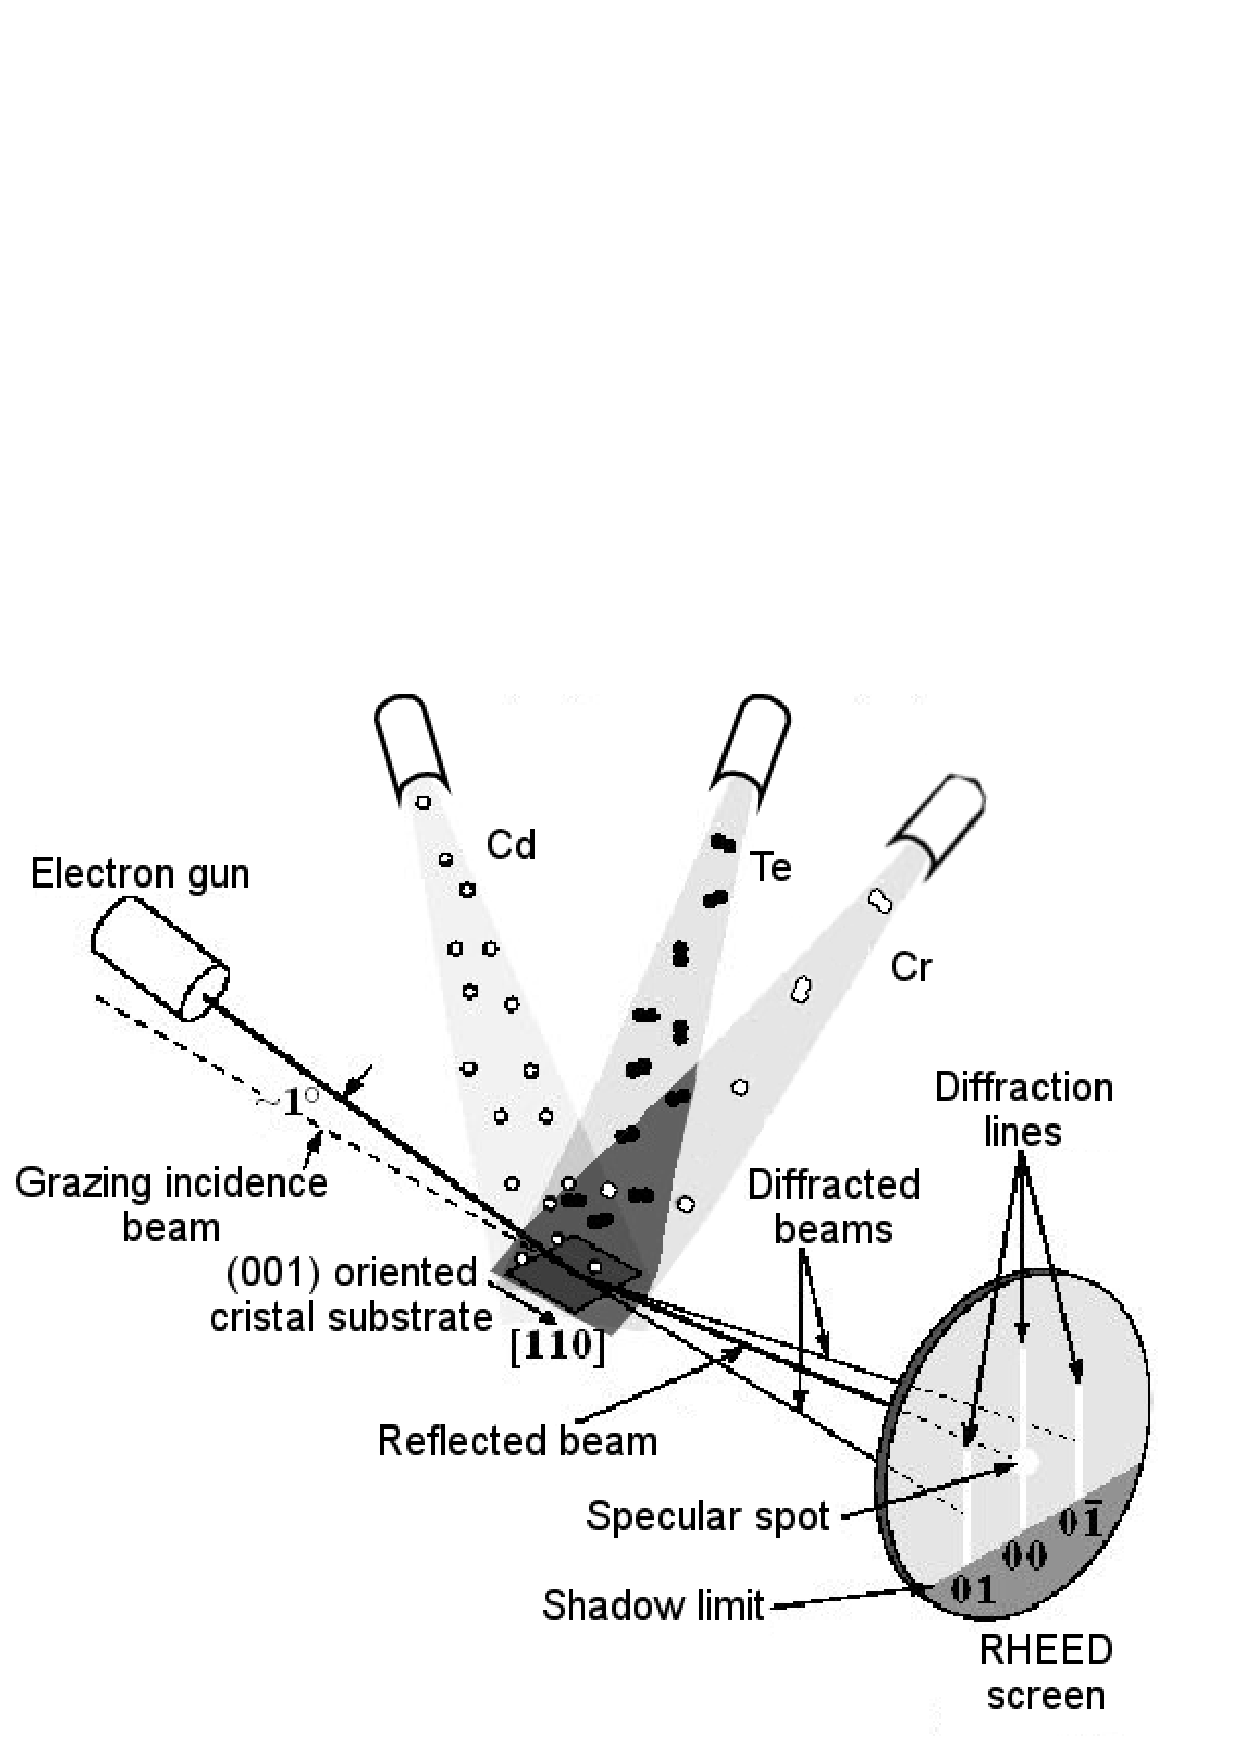
\includegraphics[width=10cm]{Pictures/MBE.png}
	\end{center}
	\caption{Scheme of a MBE chamber and the position of the cells in regard of the substrate.}
	\label{MBEScheme}
	\end{figure}
	
%	Since MBE is a slow growth process, it ask for ultra-vacuum condition, in the order of $10^{-8}$ Pa, to avoid any contamination of the sample. Each raw material is contained in a Knudsen cell, which consist of a crucibles of high-melting-point material with a low contaminating power (typically Pyrolytic Boron Nitride) wrapped in tungsten filament which will act as heater. A small shutter close the container, and is controlled by computer along each recipe sequences.
	
	This necessity of Ultra High Vacuum kept the MBE to be developed before the end of the 1960s \cite{FirstMBE}, although the the idea was formalized at the end of the 19th century. This method offers a good control on the growth, which make it useful for the development of nanostructure and nanoscience. The deposition layer by layer give the possibility to grow really thin structure, and the transition between two materials can be really abrupt, on a few monolayer (ML). Growing nano-structure is still the main use of MBE. However, this method is mainly on research purpose, its slow growth speed and hard to fulfil growth conditions being an obstacle for the industrialization of the process.
	
	Another mode of MBE is used during the growth of the samples: Atomic Layer Epitaxy (ALE) or Migration-Enhanced Epitaxy (MEE). In this mode, only one element is opened at a time, growing the sample really layer by layer. Between each opening, the sample is left under vacuum in order to relax the surface. A full cycle correspond to opening each cell once. For CdTe, a substrate temperature between 260$^{\circ}$C and 290$^{\circ}$C guaranty a growth of only 0.5 ML for each cycle~\cite{HMarALE}. This allow a small uncertainty on the substrate temperature while keeping a really good control on the growth of the sample.
	\newline
	
%	In order to monitor each step of the growth, RHEED patterns of the sample surface were taken at different key moments. 
	The growth was monitored with RHEED (Reflexion High-Energy Electron Diffraction). This technique requires a high vacuum, a given since MBE ask for ultra-high vacuum condition, and the use of an electron gun able to produce high energy electron. The beam of the gun is sent at low angle, between 1$^{\circ}$ and 3$^{\circ}$, to the surface sample. This way, the electrons will only probe the surface of the sample, entering the material only on a 3 or 4 ML. Therefore the detected pattern directly gives information on the flatness and the crystallinity of the surface.
%	The detector, a CCD camera,  is set in order to collect only elastically scattered electrons.
	
	Incident electrons have a wave vector $\mathbf{k_i} = 2 \pi / \lambda_e$, with $\lambda_e$ the electron wavelength, typically 6 or 7 pm for an electron gun energy between 30 and 40 kV. Since only scattered diffraction is considered, the diffracted wave vector $\mathbf{k_f}$ as the same norm as the incident one $\mathbf{k_i}$. So the Ewald's Sphere has a radius equal to the norm of $\mathbf{k_i}$. In the reciprocal space, the plane of diffraction are infinite line. So, in the case of a perfect crystal, with a a perfect detector, the intersection with Ewald's sphere should be points. However, since the crystal can have some defect and neither the gun or the detector are perfect, the diffracted pattern present line, such as visible on Fig.\ref{RHEEDStep}(b).
	
	Once dots are grown, though, the surface become rough at the scale of the length of coherence of the beam. The electrons can interact with several more layer while passing through the dots. This can be seen on the diffraction pattern, where lines become points, such as shown on Fig.\ref{RHEEDStep}(e).
	
	Another use of the RHEED diffraction is the monitoring of the number of layer grown through ALE. Focusing on the lowest angle reflected spot, called the specular spot, one can see small variation in the reflected intensity during the growth, such as presented on Fig.\ref{RHEEDOsc}. This intensity is minimal when there is half a ML grown, and maximal when the ML is fully grown. This is due to the variation of reflectivity of the surface: maximal for a flat surface, minimal for a rough one. Therefore, a period of these oscillation is exactly the growth of a single monolayer~\cite{FirstRHEED,WoodRHEED}. We can also see the relaxation of a layer, if the variation of intensity disappear at a point.
	
	\begin{figure}[h!]
	\begin{center}
		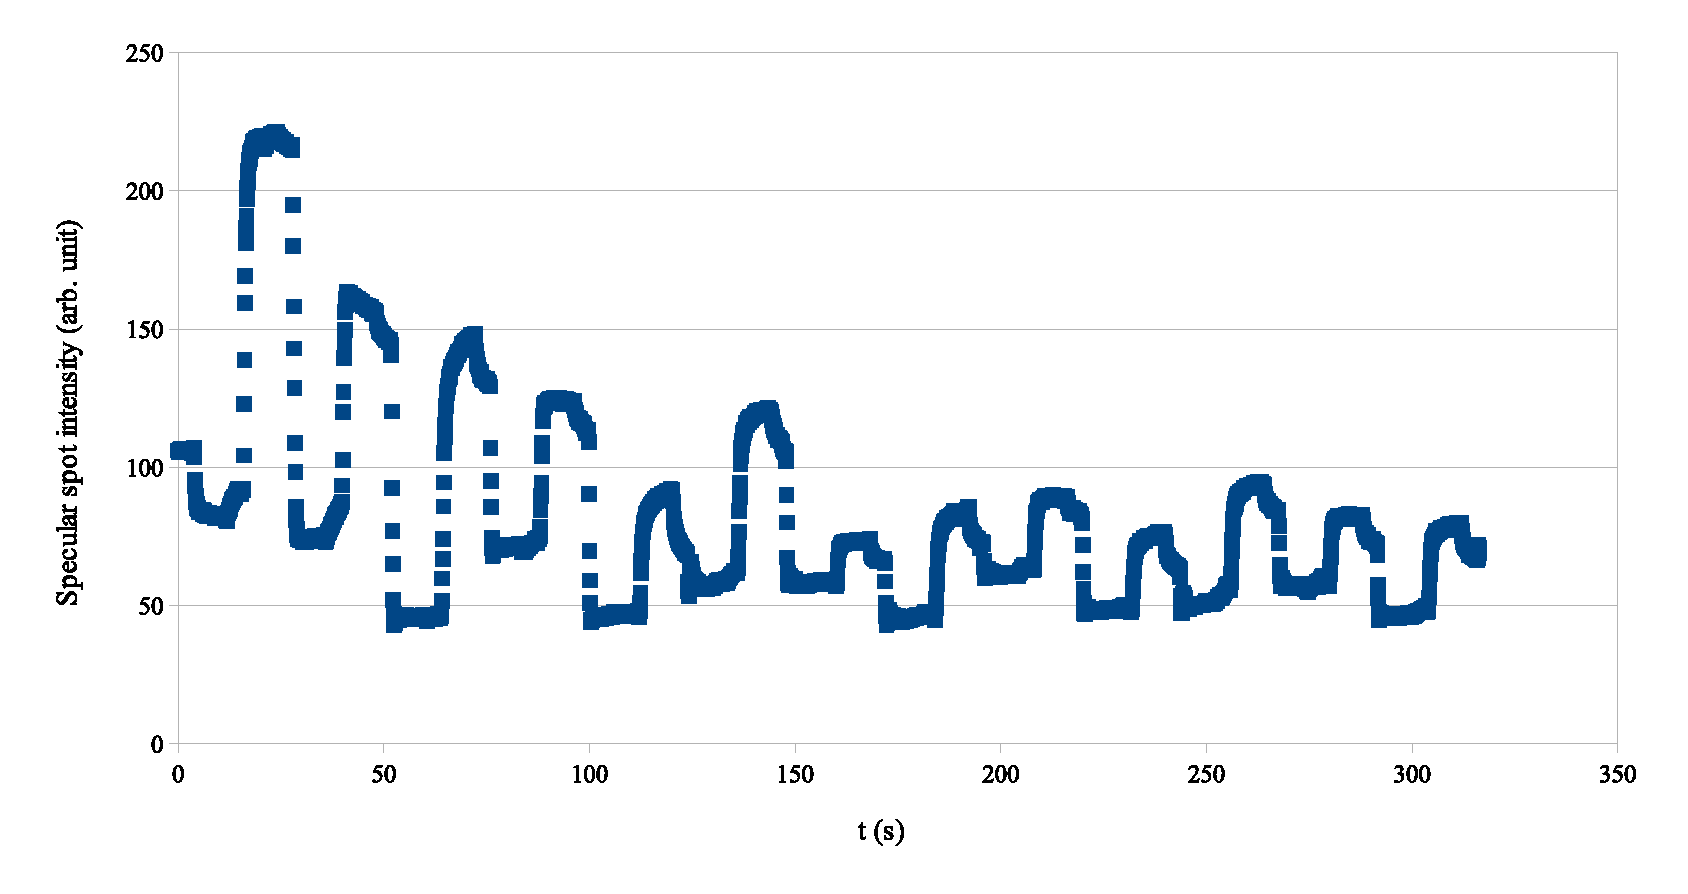
\includegraphics[width=14cm]{Pictures/SFDRheed.eps}
	\end{center}
	\caption{RHEED oscillation for the ALE of strained dots.}
	\label{RHEEDOsc}
	\end{figure}
	
	%We are working with two sample holder, named "marked" and "unmarked", with slightly different temperature offset. The thermometer to measure the substrate temperature is placed at a few centimetre from the substrate holder, inducing another offset in the measured temperature.
	
	\section{Strained dots: CdTe/ZnTE\label{SK}}
	
	\subsection{Substrate preparation}
	
		The sample was grown on ZnTe(100) substrates. In order to get the bes surface to grow on, we need to clean the sample. Two cleaning methods were tested: etching of the sample in a Bromure solution, and exposition of the sample to a hydrogen radical plasma.

		The etching process was done in four steps. All of them, except the etching in Bromure-ethanol, occur in an ultrasonic cleaning device vibrating the sample at 43kHz and last 3 minutes. We began with a cleaning in acetone, followed by one in ethanol. The third step was the actual etching: the substrate was put in a solution of Bromure-ethanol, with 3\% of Bromure, during 1 minute. We finally rinsed it in methanol. Once rinsed, we keep the sample in ethanol until fixing them to the sample holder. The growth usually occur the day after the cleaning, the sample being kept in the MBE load-lock chamber, under vacuum.
		
		Another type of cleaning of the surface was tried: using hydrogen radical (H$^*$) to remove the impurity at the surface. This was done to get a smoother surface directly in the chamber, to avoid any contamination by the atmosphere that might occur during the transport from the etching room to the MBE chamber. In order to form the radical gas, a hydrogen gas was ionized in a chamber by a RF power source of 300 W and with a frequency of 13.6 MHz. This gas composition is optically checked by probing the emission of the Balmer series: for a pure hydrogen gas, peaks at 656 nm and 486 nm appear clearly. During the formation of this gas, the substrate temperature is raised to $400^{\circ}$C and we initiate its rotation. Once the plasma is formed, the valve to the main chamber is opened and the substrate is exposed to the plasma for 15 minutes. In order to check the quality of the surface, we look at the RHEED that should present strike.
	
	\subsection{Strained dots growth\label{SKGrowth}}
	
	The targeted flux chosen for the growth of the CdTe/ZnTe QD are presented in Tab.~\ref{FluxTempSK} for each cell used during the growth of strained QDs. These flux were measured via the pressure gauge inside the MBE chamber. It was shown that the best quality of ZnTe was achieved for a growth in excess of Zn~\cite{TeEffect}. Otherwise, vacancies appear in the bulk, optically visible, and the surface is more rough. Moreover, the adsorption power of the Zn is smaller than the Te. For these reason, we choose to grow the ZnTe barriers in excess of Zn.
	
	\begin{table}[h!]
	\begin{center}		
		\begin{tabular}{| c | c |}
			\hline
			Elements & Targeted BEP (Torr) \\ \hline
			Cd & $4.5\times10^{-7}$ \\
			Te & $4.5\times10^{-7}$ \\
			Zn & $6.8\times10^{-7}$ \\
			\hline
		\end{tabular}
		\caption{Aimed flux for each cell during the growth of the strained QDs.}
		\label{FluxTempSK}
	\end{center}
	\end{table}
	
	The CdTe quantum dots was grown using ALE. When the sample is exposed to either Cd or Te, only one atomic layer will be deposited under each flux: we call this \emph{auto-regulated} growth. The flux for both of the compound are therefore chosen to be the same~\cite{HMarALE}. 
	
	Beginning the growth, the substrate temperature was initially raised to $320^{\circ}$C. The Zn cell shutter was open starting at $250^{\circ}$C, in order to flatten the surface for the growth. While it took several minutes to raise the substrate temperature, only one Zn layer was deposited due to the auto-regulation of the growth. When the substrate temperature reach $320^{\circ}$C, the Te shutter was also open, in order to grow the ZnTe buffer layer. This thick ZnTe layer guaranteed us to the best possible surface for the growth of the QD layer~\cite{ChangZnTe}. Once done, we set up the RHEED, growing a few more ZnTe level while searching the specular spot. The substrate temperature was then lowered to $170^{\circ}$C, the Zn cell being open until the temperature reach $250^{\circ}$C.
	
	\begin{figure}[h!]
	\begin{center}
		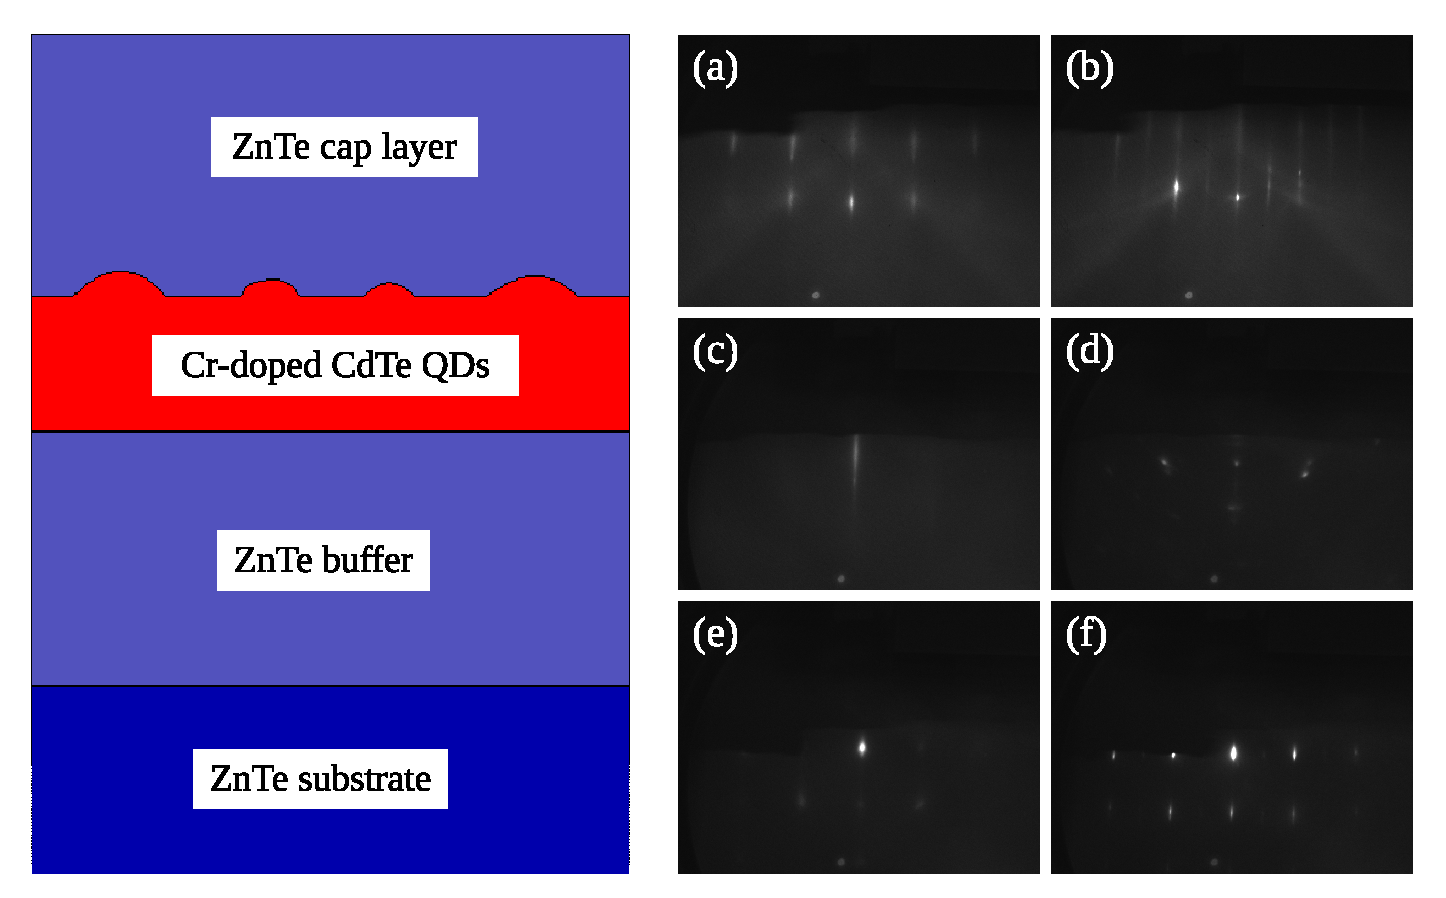
\includegraphics[width=14cm]{Pictures/RHEEDStep.eps}
	\end{center}
	\caption{Left: Layer structure of the strain Cr-doped CdTe QDs samples.
		Right: RHEED pattern taken at different key moment of the growth: (a) before the growth of the ZnTe buffer, (b) after the growth of the ZnTe buffer, (c) after the (Cd,Cr)Te ALE, (d) after the Te deposition, (e) during the Te evaporation (the picture was taken at T$_{substrate} = 177^{\circ}$C) and (f) after the growth of the ZnTe cap.}
	\label{RHEEDStep}
	\end{figure}
	
	One of the main difficulty of this work was to calibrate the Cr flux in order to embed only a single Cr atom in most of the QDs of the sample. To achieve this, the Cr density must be of the same order as the QDs density at the surface of the sample. This means a really small flux, with a BEP of the magnitude of $10^{-10}$ Torr, which is about one order lower than the main chamber pressure and therefore not measurable with our technique. The optimisation was done starting with the know how acquired in Grenoble on the Mn and trying to optimise it for the Tsukuba machine, through a feedback loop with the micro-PL characterization in Grenoble.

	This really small flux was achieved by heating the Cr cell around 1000K, low compared to its sublimation temperature, and opening the cell only once during the ALE, for only 5s. In order to have big enough QDs, emitting at right wavelengths, 6.5 ML of CdTe is the optimal CdTe thesis. However, the critical thickness of CdTe on ZnTe is 6.5 ML. Dislocations and defect will form in the layer for a higher thickness. Therefore, some sample were also grown with a 5.5 ML thickness in order to not get too close to the limit. At the chosen temperature, it correspond to either 13 cycles of ALE (for 6.5 ML) or 11 cycles (for 5.5 ML). The Cr cells was opened during the 7th cycle, halfway through the growth of the QD layer, in order to allow the Cr atoms to diffuse without going out the QD layers. The whole ALE recipe to grow the QDs layer is given in the Fig.\ref{RecipeSK}.
	
	\begin{figure}[h!]
	\begin{center}
		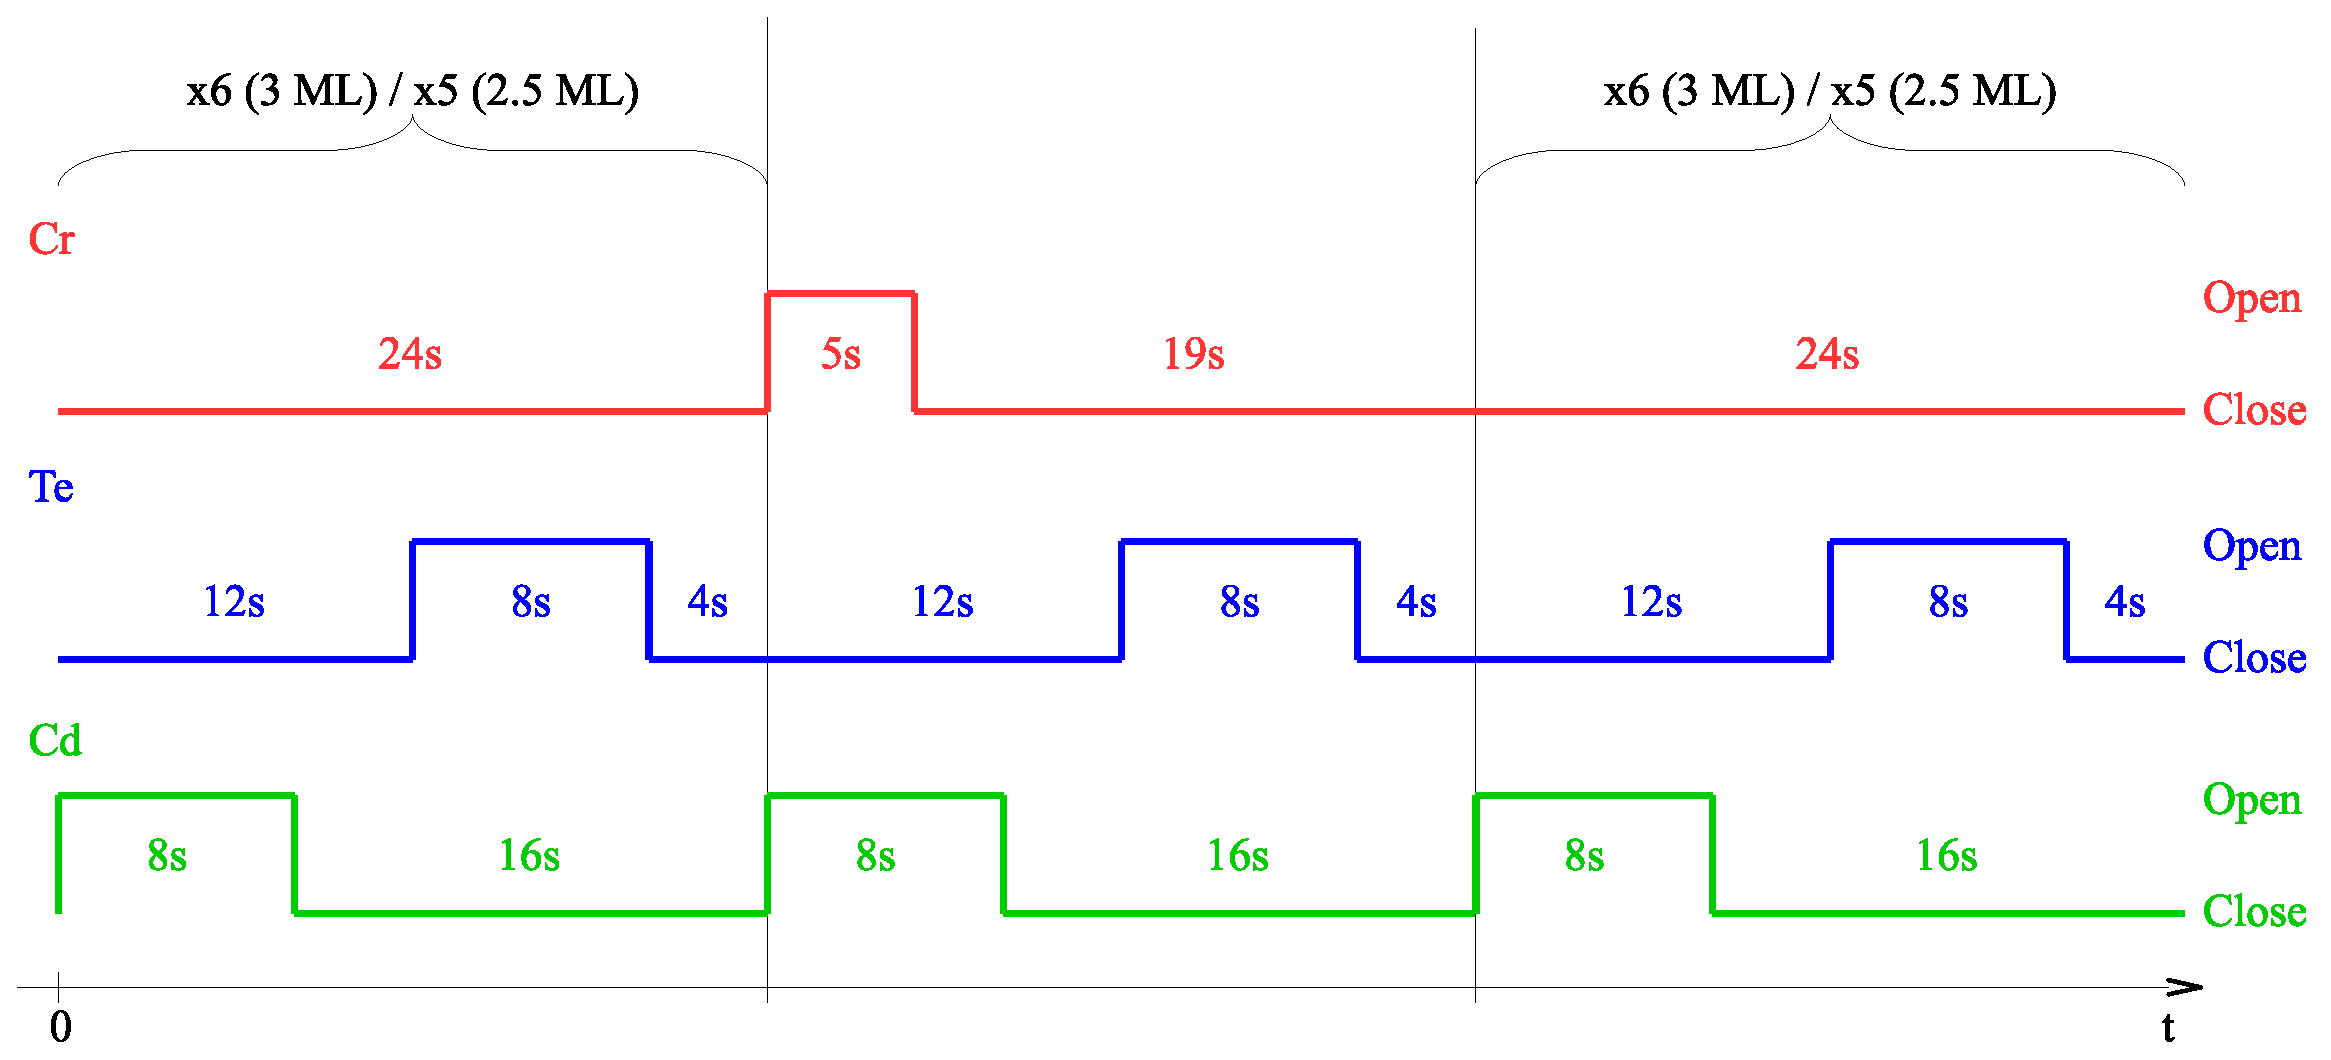
\includegraphics[width=14cm]{Pictures/RecipeSK.eps}
	\end{center}
	\caption{Opening and closing cycles of each cell for the ALE of strained (Cd,Cr)Te samples.}
	\label{RecipeSK}
	\end{figure}

	After the growth of the CdTe layer, we lowered the substrate temperature to $90^{\circ}$C to deposit the Te layer. It was deposited during 5 minutes. This step allows the CdTe layer to relax and form the quantum dots~\cite{TinjodMBE}. We then heated up the substrate again until $200^{\circ}$C, were we stayed for 20s in order to evaporate all the deposited Te~\cite{WojnarMBE}. If the dots were formed, we saw a spotty pattern like the one presented on Fig.~\ref{RHEEDStep} (f). The Zn and Te cells were then opened, while the substrate temperature was raised to $240^{\circ}$C in order to grow a protective layer above the QDs.
	
	\subsection{Results}
	
	\begin{table}
		\begin{center}
			\caption{List of samples where Cr was found.\label{Sksamples}}
			\begin{tabular}{M{2cm}|M{3cm}|M{3cm}|M{2cm}|M{3.5cm}}
				Sample & Type & Cleaning process & # CdTe MLs & Cr aimed concentration (\%) \\
				\hline
				dot358 & Br etching & Strained dots & 6.5 & 0.06 \\
				dot359 & Br etching & Strained dots & 6.5 & 0.11 \\
				dot363 & Br etching & Strained dots & 6.5 & 0.21 \\
				dot383 & Br etching & Strained dots & 5.5 & 0.19 \\
				dot385 & Br etching & Strained dots & 5.5 & 0.17
			\end{tabular}
		\end{center}
	\end{table}
	
	\lipsum[1-2]
	
	\section{Other kind of samples}
		\subsection{Charge control samples\label{ChargedSample}}	
		
	Charge control samples are pretty straightforward. Instead of growing the sample on a non-doped ZnTe substrate, we do the growth on p-doped ZnTe substrate. Same steps are followed, but with thinner buffer and cap layers, in order to have a stronger electric on the dot layer. We chose to do both about 150 nm thick, calibrating with the ZnTe growth speed calculated via the RHEED oscillations.
	
	Once the growth were finished, a thin, semi-transparent gold layer is deposited by sputtering. The samples are kept in nitrogen atmosphere during the transport. The exposition time of the sample in the sputtering machine was calibrated using gold deposited on GaAs substrate. Resistance of the gold layer was measured. Results are presented in Fig.~\ref{AuDep}. In order to keep a collection of the light emitted by the quantum, a thin layer was necessary. However, we also needed a gold layer thick enough to cover the entire surface of the sample. These considerations lead us to chose a deposition time of 35 s.
	
	\begin{table}
%		\begin{center}
			\fcapside{\caption{Measured conductivity of the Au layer on GaAs for different deposition time.}\label{AuDep}}
			{\begin{tabular}{M{3cm}|M{2cm}}
				Gold deposition time (s) & Resistance ($\Omega$) \\
				\hline
				15 & 300 \\
				20 & 80 \\
				25 & 25 \\
				30 & 20 \\
				35 & 0 \\
				60 & 0
			\end{tabular}}
%		\end{center}
	\end{table}
	
	\subsubsection*{Results}
	
	\lipsum[1]
	
	\begin{figure}[h!]
	\begin{center}
		\includegraphics[width=10cm]{../FillingPicture.png}
	\end{center}
	\caption{Example of charge variation}
	\label{ChargeVar}
	\end{figure}
	
	Only one charged sample containing Cr atoms was grown: dot390. It was cleaned by H$^*$ plasma. The QD layer was 5.5 ML thick and the Cr concentration was aimed to be 0.16\%. However, no Cr doped quantum dots were found. Some dots presenting a emission close to the one expected for Cr atoms were found, but they were revealed to not have any magnetic atom inside. These are discussed in more in Sec.~\ref{ChargeFluc}.
	
		\subsection{Strain-free quantum dots\label{SFD}}
		
%		The strain-free dots are formed by the interface variation of a thin (about $4ML$) CdTe quantum well (QW) between CdMgTe layers. These thickness variations will create dots, in which we will want to include a single magnetic atom. The whole structure is ideally grown on a CdTe substrate, in order to have absolutely no strain in the dots layer.
%		
%		However, there was no CdTe substrate in Tsukuba. So, we had to grow a thick layer of CdTe in top of GaAs substrate, which a lattice parameter close to CdTe, on order to have a completely relaxed surface to do our growth.
%		
%		To achieve so, we start by cleaning the GaAs substrate. It was done in four step outside the MBE chamber, all of them using an ultrasonic cleaning. It was first immersed in acetone, during 5 minutes, with the ultrasonic frequency at $43MHz$. Staying at this frequency, it was then immersed in ethanol during 5 minutes again, and then in water for the same time. We finished with a last 5 minutes cleaning in water, at $23MHz$ this time.
%		
%		Putting the substrate in a chamber, we proceeded to the last step of the cleaning: hydrogen radical (H$^*$) cleaning, created by injecting nitrogen radical in a chamber of H gas, in order to remove Ga oxyde formed at the surface while transporting the sample. We check the final composition of the gas via the electron energy using optical probing. For a H$^*$ gas, this should be round 660nm. To achieve the H radical cleaning, we heat the GaAs substrate to $400^{\circ}$C and then open the valve between the main chamber and the one containing H$^*$ gas. We exposed it for 15 minutes, and then searched for line in the RHEED pattern, to check the quality of the cleaning. during this step, and also during the growth, the sample was rotating.
%		
%		Once the cleaning process is finished, we began the growth of the thick layer of CdTe. We began by a very thin layer of ZnTe in order to relaxed some of the strain. Staying at T$_{substrate} = 400^{\circ}$C, we first opened the Zn cell for 30s, then opened both Zn and Te cells for 50s, before closing again Te cell. We then go down to T$_{substrate} = 250^{\circ}$C under Zn flux and, once the temperature was stabilized, closed the Zn cell and proceeded to the CdTe layer growth, during 1h. Finally, once this layer was grown, we protected it from oxidation by adding a thin layer of Te while the substrate temperature was going down to $5^{\circ}$C.
%		
%		For this sample, only a simple cleaning occur outside of the MBE machine. We did it in four steps, each of them lasting for 5 minutes in an ultrasonic cleaning device. We began with a cleaning acetone, at 43 kHz, followed by one in ethanol at the same frequency. We then put the substrate in water and clean it at 43 kHz. Finally, we changed the water and did the last step in water at 23 kHz, in order to clean the substrate from smaller dust particle.
%		
%		Since the surface of the GaAs is oxidized, no RHEED pattern was visible, as shown on Fig \ref{Hybrid}(a). The desoxidation was done in the MBE main chamber, in vacuum condition, using hydrogen radical (H$^*$). In order to form the radical gas, a hydrogen gas was ionized in a chamber by a RF power source of 300 W and with a frequency of 13.6 MHz. This gas composition is optically checked by probing the emission of the Balmer serie: for a pure hydrogen gas, peaks at 656 nm and 486 nm appear clearly. During the formation of this gas, the substrate temperature is raised to $400^{\circ}$C. Once the hydrogen chamber is full of H$^*$ gas, we initiate the rotation of the sample. Since the chamber was situated just under the main and linked to her, we just had to open the shutter between the two to send the radical gas onto the substrate. We exposed the substrate to this gas for 15 minutes, under a pressure of about $6\times10^{-7}$ Torr. We then checked the sample surface with RHEED, which should present a streak pattern with some dots as presented in Fig \ref{Hybrid}(b). 
%		
%		Once the cleaning of the sample was finished, we closed the H$^*$ gas chamber shutter, waited for the ultra-high vacuum to re-established in the main chamber and began the growth of the CdTe layer. We grew it in two times: one hour of growth just after the cleaning (described here) and about four hours just before the actual growth of  the quantum dots structure.

%	The barrier for strain free samples are made of CdTe. The chosen substrate for the growth was GaAs, on which we grew a layer of about 3 $\mu$m of CdTe. Growing such a thick layer guaranty that the remaining strain are in the order of $0.1\%$ \cite{StrainRelaxCdTeGaAs111,StrainRelaxCdTeGaAs100}. Moreover, a small ZnTe layer was grown between GaAs and CdTe, which accelerated the relaxation of the strains \cite{StrainRelaxZnTeGaAs001}.
	
	Strain-free quantum dots are formed by the thickness fluctuations of a CdTe quantum well in Cd$_x$Mg$_{1-x}$Te barriers. These fluctuations form steps localizing the carrier, acting as QDs. The higher the Cd concentration will be, the closer the lattice parameter will be, but it will also reduce the gap energy difference, reducing the confinement. The best strain to confinement ratio was found for CdTe QW in Cd$_{0.7}$Mg$_{0.3}$Te. The needed flux for this growth are shown in Tab.~\ref{FluxTempSFD}.
	
	\begin{table}[h!]
	\begin{center}		
		\begin{tabular}{| c | c |}
			\hline
			Elements & Targeted BEP (Torr) \\ \hline
			Cd & $4.5\times10^{-7}$ \\
			Mg & $1.6\times10^{-8}$ \\
			Te & $5.26\times10^{-7}$ \\
			\hline
		\end{tabular}
		\caption{Aimed flux for each cell during the growth of the strained samples.}
		\label{FluxTempSFD}
	\end{center}
	\end{table}
	
	The strain-free sample were grown on an hybrid substrate. The substrate was made from a GaAs substrate, cleaned using H$^*$ plasma. We grew on it a CdTe layer of about 3 $\mu$m, in order to recover the lattice parameter and not have defect close to the surface. With this thickness, the remaining strain in the layer should be of about $0.1\%$~\cite{StrainRelaxCdTeGaAs111,StrainRelaxCdTeGaAs100}. A thin layer (about 7 nm) of ZnTe was grown between the GaAs and the CdTe in order to help the relaxation of strains~\cite{StrainRelaxZnTeGaAs001}. The RHEED taken after the growth of the CdTe layer (Fig.~\ref{Hybrid} (d)) shows sharp straight line, hinting at the recovery of a flat surface. A protective layer of amorphous Te was grown on the surface to keep it from being damaged outside the MBE chamber. It was removed at the beginning of the growth by evaporation.

	\begin{figure}[h!]
	\begin{center}
		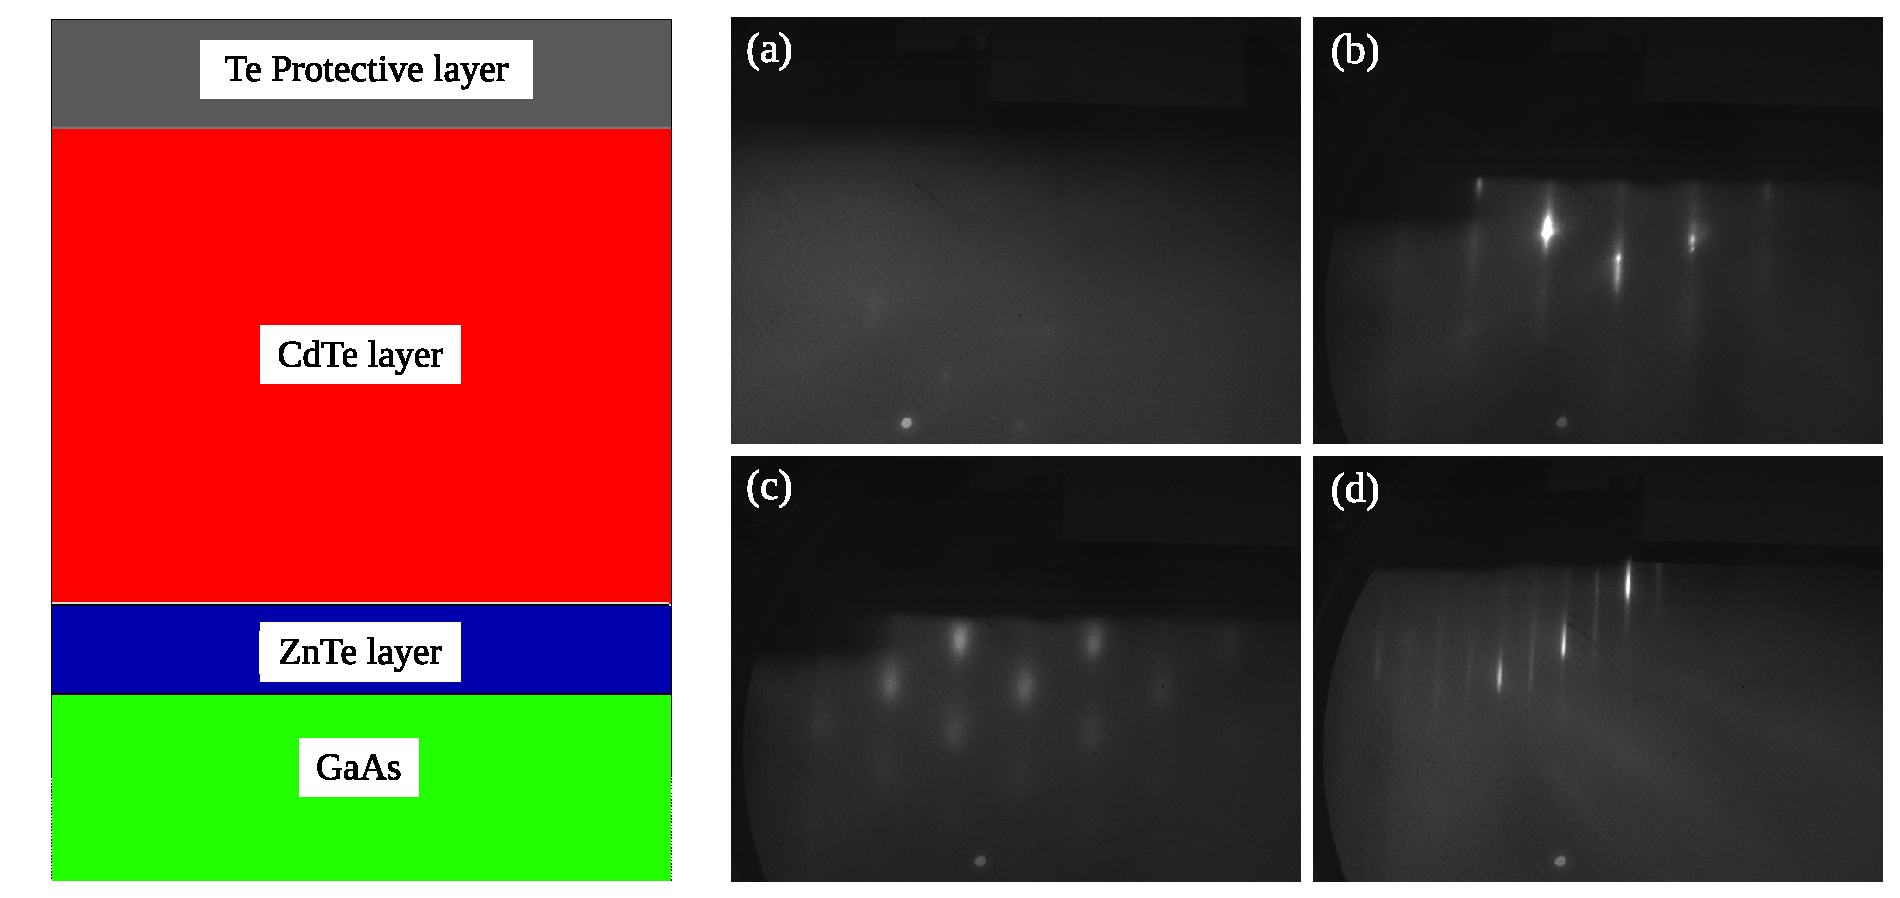
\includegraphics[width=14cm]{Pictures/HybridSubstrate.eps}
	\end{center}
	\caption{Left: Layer structure of the hybrid substrate with its protective Te cap.
		Right: RHEED pattern taken at different key moment of the growth: (a) before H$^*$ cleaning of GaAs, (b) after H$^*$ cleaning of GaAs, (c) after the growth of the ZnTe layer, (d) after the growth of the CdTe layer.}
	\label{Hybrid}
	\end{figure}
		
%		This first part of the growth took place on a rotating sample. It only take about 15 ML of ZnTe on GaAs for the II-VI compound go back to its original lattice parameter \cite{StrainRelaxZnTeGaAs001}. Moreover, CdTe over ZnTe has a critical thickness of 5 ML \cite{CritThickCdTeZnTe}. So, to accelerate the relaxation of strain, we decided to grow a thing layer of ZnTe above the GaAs, before growing the CdTe thick layer. We lowered the substrate temperature to $320^{\circ}$C and opened the Zn cells for 30s with a BEP of $7.05\times10^{-7}$ Torr in order to flatten the surface. We then opened the Te cells, with a BEP of $5.21\times10^{-7}$ Torr, along with the Zn cell during 50s to grow the ZnTe layer in excess of Zn, making a layer about 7.2 nm thick.
%		
%		We then went to the growth of the first CdTe layer. We lowered again the substrate temperature to $250^{\circ}$C, under Zn flux. Once stabilized at the temperature, we closed Zn cells and open the Cd and Te cells for 1h. The Te cell had the same flux as previously, while the Cd cells had a flux of $4.72\times10^{-7}$ Torr. This layer was 633 nm thick, grown at 0.54 ML.s$^{-1}$. In order to protect the surface, we deposit an amorphous protective layer of Te above it, while decreasing the substrate temperature.
		
%	As said in the introduction, the strain free dots are formed by thickness variation of a CdTe QW surrounded by CdMgTe barrier. In order to have to good confinement while keeping a close enough lattice constant, we chose to use Cd$_{0.7}$Mg$_{0.3}$Te. Therefore, the first step of the growth was to chose the flux for the growth. We went through a process of trial and error, growing several samples and testing their composition with Electron Probe Mico-Analysis and X-Ray diffraction, as well as the thickness grown with a step gauge, in order to estimate the growth speed. Since we wanted to grow Cd$_{0.7}$Mg$_{0.3}$Te, we began the test with a ration Te:Cd of 1:0.7 and a ratio Te:Mg of 1:0.3. After five round of adjustment, we achieve the growth of Cd$_{0.7}$Mg$_{0.3}$Te, settling with the targeted flux presented in Tab.\ref{FluxTempSFD}.
%	For the settled Mg flux, the step gauge indicated a grown thickness of $520 \pm 5$ nm. Since we grew the test layer during 1h, we found a growing speed of about 0.15 nm.s$^{-1}$.
	
	We began to heat the substrate temperature to 180$^{\circ}$, in order to remove the protective amorphous Te layer. We waited a few second at this temperature to remove all the deposited Te, and then resumed the heating to go to $250^{\circ}$C. Starting at $200^{\circ}$C, we opened the Te cells in order to stabilize the surface. When the substrate temperature was stabilized at $250^{\circ}$C, we opened the Cd cells and grew a 2.35 $\mu$m layer of CdTe, in order to be as close as possible of a total lattice parameter recovery ~\cite{StrainRelaxCdTeGaAs111,StrainRelaxCdTeGaAs100}.
	
	We grew the first Cd$_{0.7}$Mg$_{0.3}$Te barrier on this buffer layer. In order to be sure that there will be no relaxation in the quantum well, we choose to stick to the maximum cumulated thickness of the CdTe on a CdZnTe lattice, which has been shown to be lower than the one of CdTe on a CdMgTe lattice. This correspond to a maximum cumulated thickness of 130 nm \cite{CritThickCdTeCdZnTe}. We chose to grow 40 nm below the QW, and 90 nm above it, in order to have a thicker protective layer.
%Moreover, it was shown on Mn that a thick layer above was better for the hole trapping.

	Once the 40 nm barrier layer was grown, we lowered the substrate temperature under Te flux. Growing the QW layer in a Te environment smooth the surface layer of the sample and help having a flat surface to grow the well. Once the substrate temperature reach respectively $170^{\circ}$C, we began the ALE of the QW. Two QW thickness was tested: either 4 ML or 2 ML. In both case, the growth was done growing CdTe layer as done for the strained sample, opening the Cr cell for 3 s for one cycle every two cycle. The whole recipe is described in Fig.\ref{RecipeSFD}.

	\begin{figure}[h!]
	\begin{center}
		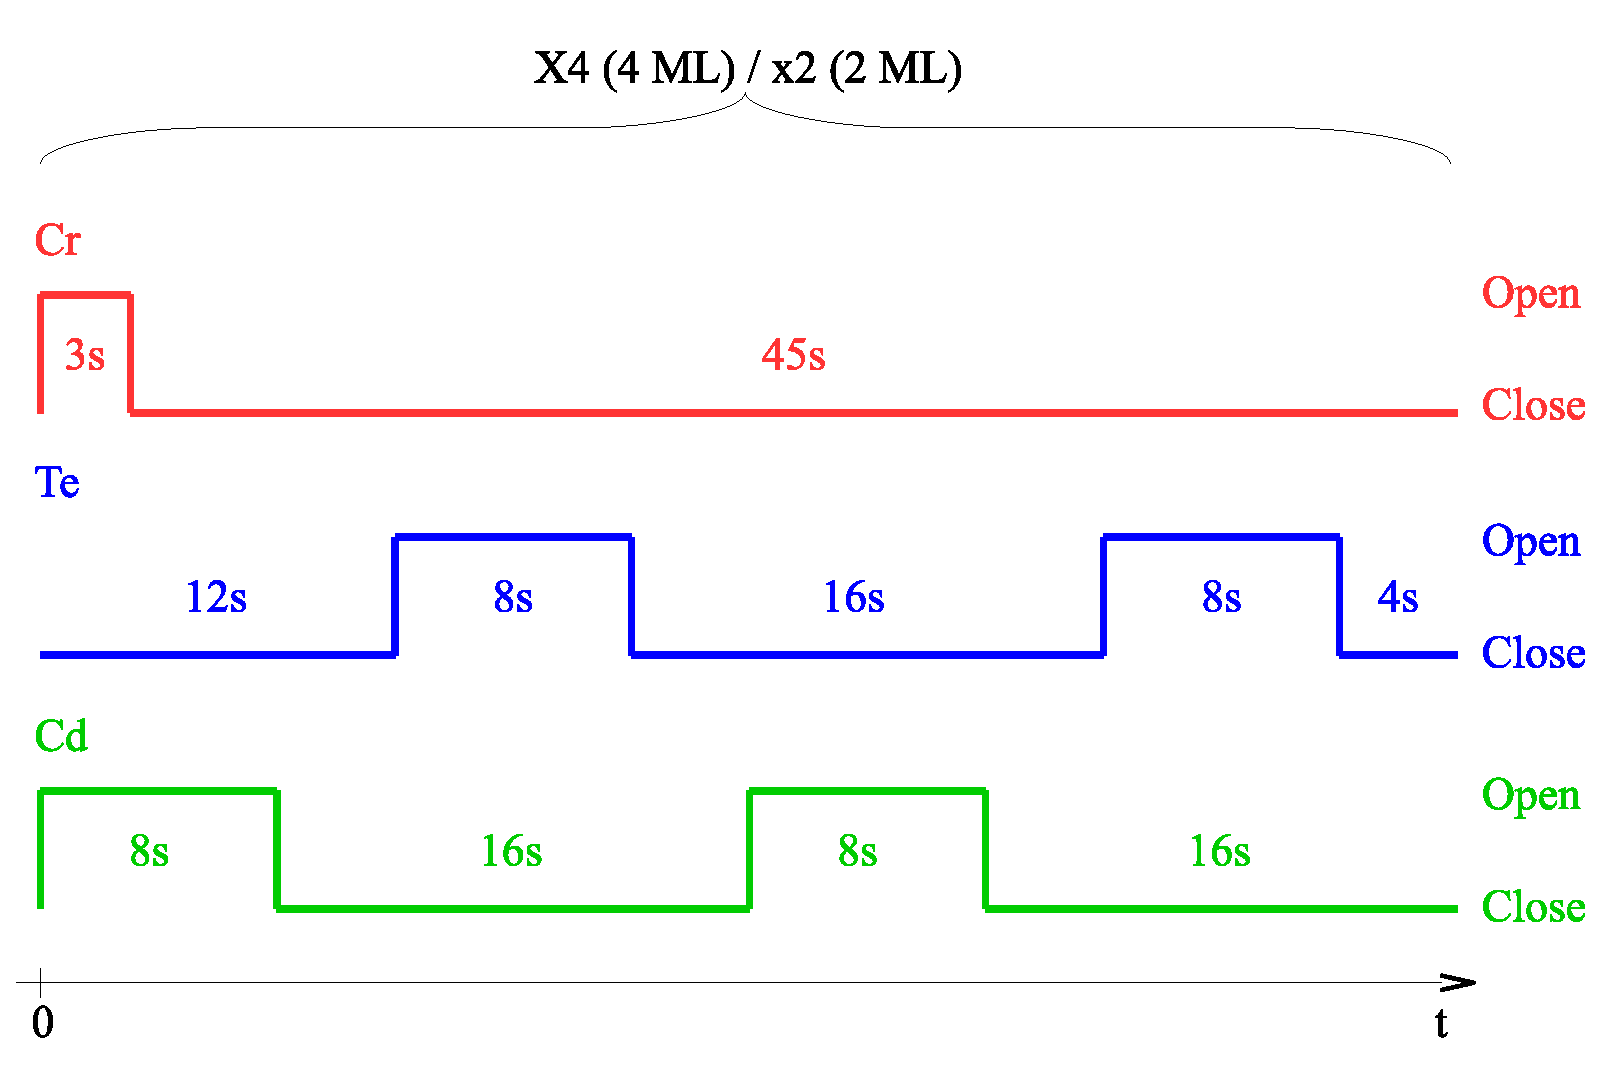
\includegraphics[width=10cm]{Pictures/RecipeSFD.eps}
	\end{center}
	\caption{Opening and closing cycles of each cell for the ALE of strain free (Cd,Cr)Te samples.}
	\label{RecipeSFD}
	\end{figure}
	
	We then raised the substrate temperature up to $250^{\circ}$C, under a Te flux, in order to proceed to the growth of the upper barrier, acting also as a protective layer. The opening time was there calculated to grow 90 nm of Cd$_{0.7}$Mg$_{0.3}$Te.

	\subsubsection*{Results}
	
	Four sample of strain-free dots doped with Cr were produced, listed in Tab.~\ref{SFDsamples}.
	
	\begin{table}
		\begin{center}
			\caption{List of sample grown trying to incorporate Cr in SFD dots.\label{SFDsamples}}
			\begin{tabular}{M{2cm}|M{2cm}|M{3.5cm}|M{3cm}}
				Sample & # CdTe MLs & Cr aimed concentration (\%) & Probability of Cr-doped QD \\
				\hline
				SFD4 & 4 & 0.35 & None found \\
				SFD5 & 2 & 0.15 & None found \\
				SFD6 & 2 & 0.54 & None found \\
				SFD7 & 2 & 0.35 & None found \\
				SFD8 & 2 & 0.75 & None found
			\end{tabular}
		\end{center}
	\end{table}
	
%	\begin{figure}[h!]
%	\begin{center}
%		\includegraphics[width=10cm]{../FillingPicture.png}
%	\end{center}
%	\caption{Example of dot fin in SFD}
%	\label{ChargeVar}
%	\end{figure}
	
	The sample presented thin and intense peaks. It hints at a better confinement of the carriers in the QDs than what have been expected from dots formed by the thickness variation of a quantum well. This may be caused by higher steps than expected at the CdTe/Cd$_{0.7}$Mg$_{0.3}$Te interface.
	
	As discussed in Sec.~\ref{XMn}, the presence of a magnetic atom split the emission of the exciton into several peaks, the number depending on the spin of the magnetic atom. However, such complex wasn't found in the strain-free samples. It may be caused by the the absence of static Jahn-Teller effect. In strain dots, this effect increase the probability of the Chromium to have a quantization axis the growth axis, $z$, making the splitting visible in our experimental setup. Without strain, the Jahn-Teller effect doesn't discriminate anymore between the three different axis, and thus the Chromium spin might have a quantization axis along the $x$ or $y$. In this case, no splitting are visible for the quantum dot in our experimental setup, and the magnetic atom goes undetected.
	
	In order to counter that, it was proposed to slightly strain the quantum well. This might be done by incorporating a low density of Zn in the Cd$_{0.7}$Mg$_{0.3}$Te barrier. The strains created this way should be enough to increase the probability of quantization along the $z$ axis, while staying negligible in regard of the Cr spin energy structure and dynamics. Such samples should be grown in the near future.

\printbibliography

\end{document}